\documentclass[10pt]{scrartcl}

% \usepackage{auto1}
\usepackage{MyriadPro}
\renewcommand{\familydefault}{\sfdefault}

\usepackage{beramono}


\usepackage[margin=0.5in]{geometry}

\usepackage{tikz}
\usetikzlibrary{shapes}
\usetikzlibrary{arrows}
\usetikzlibrary{decorations}
\usetikzlibrary{snakes}

\usepackage{fancyvrb}

\pagestyle{empty}


\newcommand{\ttffile}{\texttt{\$TTF\_FILE}}
\newcommand{\encfile}{\texttt{\$ENC\_FILE}}

\begin{document}

% ============================================================================
% 1st page
% ============================================================================
\section*{What you need to do}

\subsection*{What you need to have}
\begin{itemize}
\item A TTF file (called \ttffile from now).
\item An encoding file (called \encfile from now). Some encodings (such as \dots) are delivered  with a standard \LaTeX installation. You might want to get T1-WGL4.enc from the web.
\item The routines ttf2afm, afm2tfm, and vptovf. For debugging \dots may come in handy as well.
\end{itemize}

\subsection*{What you need to do}

\subsubsection*{What we want to generate}
\begin{itemize}
\item a MAP file
\item an FD file
\item a TFM file
\item a raw TFM file
\end{itemize}

\subsubsection*{How we do it}

% Okay, so you have your \texttt{<my-ttf-file>.ttd} and want to use in \TeX or \LaTeX? Not a big problem anymore, because pdflatex can handle TTF font files natively. That said, we need to generate a few extra helping files to enable \LaTeX to make really use of all the great features (such as kerning, ligature formation, and so on). This is what you got to do:
\begin{enumerate}
\item Come up with a proper \TeX name for your font. -- Creativity is not recommended. Please refer to http://www.tug.org/fontname/html/ There, some basic rules are suggested:
\begin{itemize}
\item The first letter corresponds to the publisher of the font (e.g., p--Adobe,\dots).
\item Positions 2,3 correspond to the actual name of the font family, e.g. fr for Frutiger, un for Univers,\dots
\item Positions 4-- specify the font, e.g. r for regular, ro for regular-oblique, bc for bold-condensed,\dots
\item The last to positions are commonly reserved for the encoding.
\end{itemize}
You can, however, name your font my\_fancy\_fontname without any harm done except being less proffessional. \mbox{\$TEXFONTNAME}

\item Next, we generate the raw TFM file, the MAP file, and -- as an intermediate product, a VPL file. On the command line, type
\begin{Verbatim}
ttf2tfm "$TTF_FILE" -q -T "$ENC_FILE" -v "$VPL_FILE" "$RAW_TFM_FILE" >> "$MAP_FILE"
\end{Verbatim}
or 
\begin{Verbatim}
ttf2afm -e "$ENC_FILE" -o "$AFM_FILE" "$TTF_FILE" 2> /dev/null
afm2tfm "$AFM_FILE" -v "$VPL_FILE" -T "$ENC_FILE" "$RAW_TFM_FILE" | sed "s/<$ENC_FILE/<$TTF_FILE <$ENC_FILE/" >> "$MAP_FILE"
\end{Verbatim}
The functions of the files within TeX are the following:

\begin{tabular*}{0.8\textwidth}{cc}
TFM file & Defines the bounding box of a glyph (that is, an atomic text element such as a letter (f,T,R) or more complex things (as ligatures, ffi, ---)). This information is used by \TeX for the actual type-setting spacing between letters and words.\\
VPL file & Contains ligature and kerning information.

If you type 'fi' in your \TeX document, \TeX will to a lookup in the ligature table and find that 'f' and 'i' are typeset as one text atom, that is the ligature 'fi' {f}{i} (watch closely here).

The kerning table tells \TeX how to correct the spaces between certain characters. This is necessary as certain letter combinations look a bit too wide apart, such as {V}A o {T}o (compare to (VA, To).

If you like, you can actually open VPNfile with a text editor and try to make sense of the entries
\end{tabular*}


\item \TeX uses a compressed version of the VPL file with the default extension VF. Hence, convert:
\begin{Verbatim}
vptovf "$VPL_FILE" "$VF_FILE" "$TFM_FILE" > /dev/null
\end{Verbatim}
The VPL file can be deleted now
\begin{Verbatim}
rm -f "$VPL_FILE"
\end{Verbatim}

\item To generate the entry in the FD file, append
\begin{Verbatim}
\DeclareFontShape{$ENC_NAME}{ua1}{$WEIGHT} {$SHAPE} {<-> $TEXNAME } {}
\end{Verbatim}

\item The last thing we need to do is move the files into the \TeX tree and update \TeX's cache. 

\end{enumerate}
% ============================================================================
% END 1st page
% ============================================================================

\newpage


% ============================================================================
% 1st page
% ============================================================================
\section*{Testing the font}
\subsection*{\dots in \TeX}
Print a nice character table with pure \TeX (not \LaTeX). On the command line, type
\begin{Verbatim}
pdftex testfont
\end{Verbatim}
give TEXFONTNAME as input, type 
\begin{Verbatim}
*\sample
[...]
*\bye
\end{Verbatim}
This returns a table with all glyphs and a sample text in testfont.pdf. The glyphs are numbered in octal notation (leftmost column) as well as hexadecimal notation (rightmost column). The order of appearence of the glyphs is uniquely defined by the encoding; can you verify this by comparing the ENCFILE with the table?

In case some glyphs don't come out quite right in the \emph{sample text}, don't worry about it: \LaTeX will probably not have any problems.

\subsection*{\dots in \LaTeX}

Use the font in \LaTeX with DeclareFont*; an example test file could look like
\begin{Verbatim}
\documentclass{article}
\DeclareFontFamily{T1}{auto1}{}
\DeclareFontShape{T1}{auto1}{m}{n}{ <-> ua1ri8t }{}
\begin{document}
\fontencoding{T1}\fontfamily{auto1}\fontseries{m}\fontshape{n}\selectfont
Some test text here.
Common ligatures: ff, --.
Common kernings: Ta, {T}a, VA, {V}A.
\end{document}
\end{Verbatim}
Does this compile without errors or warnings? Do kernings and ligatures work?

\section*{Being lazy}
% \begin{itemize}
 Of course, you don't want to declare a font in each separate \LaTeX document. That's why we are going to move it into another file, FDFILE. It's contents might look like
\begin{Verbatim}
\ProvidesFile{T1ua1.fd}
  [2008/08/14 Provides font definitions for T1/ua1.]

  \DeclareFontFamily{T1}{ua1}{}

  \DeclareFontShape{T1}{ua1}{c} {itlf} {<-> ua1cij8t } {}
  \DeclareFontShape{T1}{ua1}{c} {itsc} {<-> ua1cic8t } {}
  \DeclareFontShape{T1}{ua1}{c} {it} {<-> ua1ci8t } {}
  \DeclareFontShape{T1}{ua1}{c} {lf} {<-> ua1cj8t } {}

\endinput
\end{Verbatim}
Update \TeX's cache again, and this
\begin{Verbatim}
\documentclass{article}

\begin{document}
  \fontencoding{T1}\fontfamily{auto1}\fontseries{m}\fontshape{n}\selectfont
  Some test text here.
  Common ligatures: ff, --.
  Common kernings: Ta, {T}a, VA, {V}A.
\end{document}
\end{Verbatim}
and this
\begin{Verbatim}
\documentclass{article}

\RequirePackage[T1]{fontenc}
\renewcommand{\rmdefault}{ua1}

\begin{document}
  Some test text here.
  Common ligatures: ff, --.
  Common kernings: Ta, {T}a, VA, {V}A.
\end{document}
\end{Verbatim}
should compile. The latter is quite handy, but if you want to be even more lazy (which is a good thing to be with computers), you could create your own style file
\begin{Verbatim}
\ProvidesPackage{auto1}
[2008/07/25 J. Doe LaTeX package loading Auto 1 TTF font]

\RequirePackage[T1]{fontenc}
\renewcommand{\rmdefault}{ua1}

\endinput
\end{Verbatim}
and then simply go like
\begin{Verbatim}
\documentclass{article}

\usepackage{auto1}

\begin{document}
  Some test text here.
  Common ligatures: ff, --.
  Common kernings: Ta, {T}a, VA, {V}A.
\end{document}
\end{Verbatim}
It can't be easier than that!

% \end{itemize}
% ============================================================================
% END 1st page
% ============================================================================

\newpage

\centering

% ============================================================================
% END 1st page
% ============================================================================
\section*{\TeX's workflow}

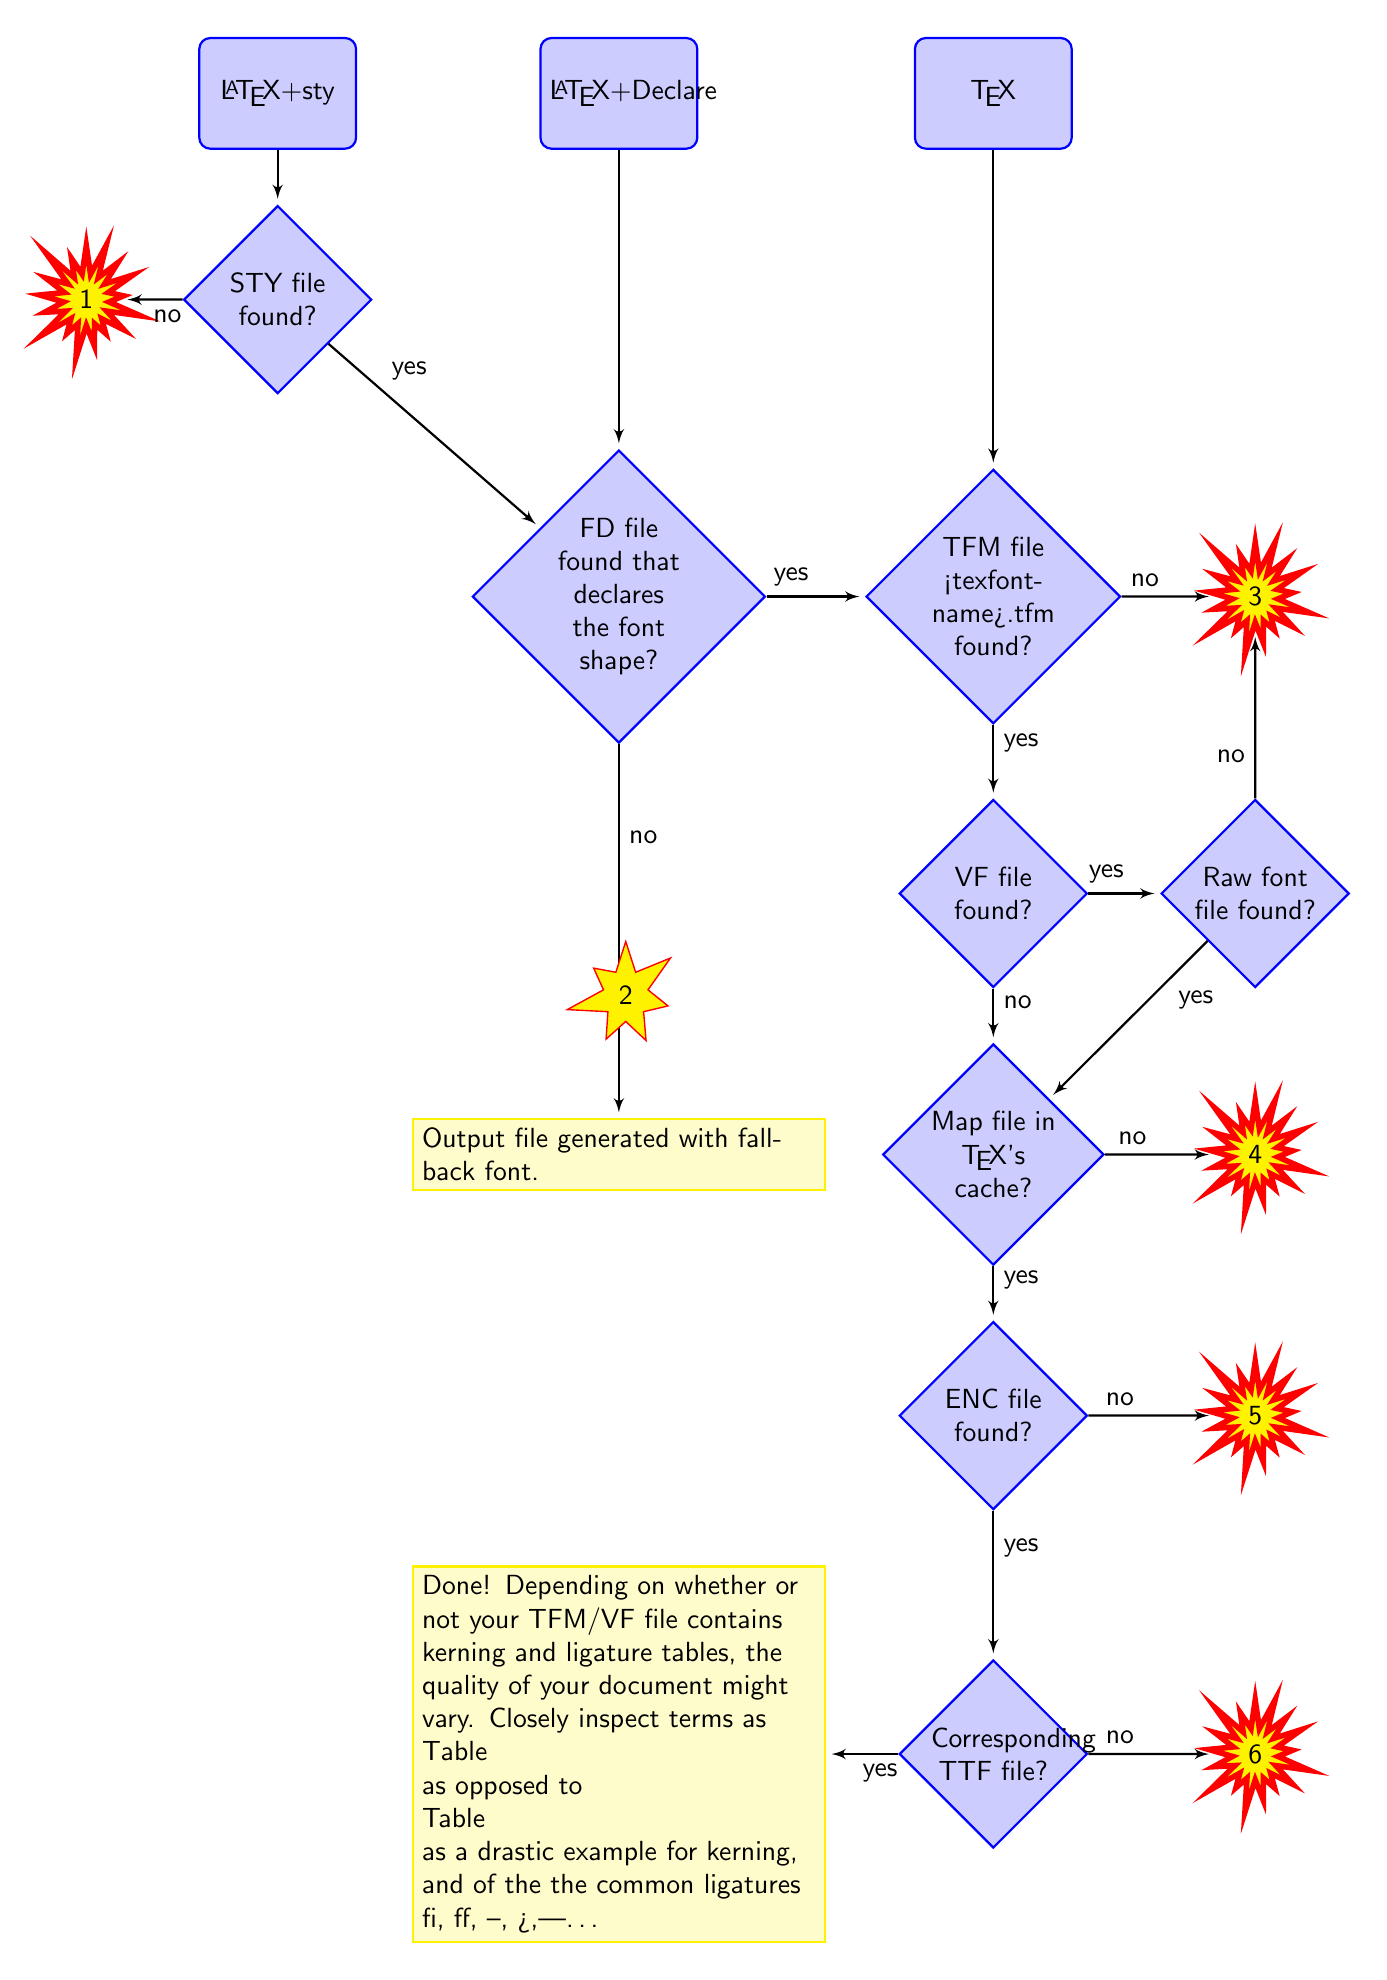
\begin{tikzpicture}
[auto,
decision/.style = {diamond, draw=blue, thick, fill=blue!20, text width=4.5em, text badly centered,inner sep=1pt},
block/.style    = {rectangle, draw=blue, thick, fill=blue!20, text width=5em, text centered, rounded corners, minimum height=4em},
line/.style     = {draw, thick, -latex',shorten >=2pt},
error/.style    = {draw=red, thick, fill=red!20, minimum height=2em},
error_number/.style  = {starburst, fill=yellow, draw=red, line width=2pt,starburst points=17},
warning_number/.style  = {starburst, fill=yellow, draw=red, line width=0.5pt,starburst points=7},
output_flaw/.style   = {draw=yellow, thick, fill=yellow!20, text width=5cm,minimum height=2em},
output/.style   = {draw=green, thick, fill=green!20, minimum height=2em}
]

% \node[starburst, fill=yellow, draw=red, line width=2pt] {\bf BANG!};


\matrix [column sep=5mm,row sep=7mm]
{
% row 0
&
\node [block] (sty_latex) {\LaTeX +sty};&
\node [block] (declare_latex) {\LaTeX+Declare};&
\node [block] (tex) {\TeX}; \\
% row 1
\node [error_number] (no_sty) {1};&
\node [decision] (sty_exist) {STY file found?};\\
% row 2
&
% \node [error_number] (no_fd) {2};
&
\node [decision] (fd_exist) {FD file found that declares the font shape?}; &
\node [decision] (tfm_exist) {TFM file <texfontname>.tfm found?};&
\node [error_number] (no_tfm) {3};\\
% row 3
&&&
\node [decision] (vf_exist) {VF file found?}; &
\node [decision] (rtfm_exist) {Raw font file found?};\\
% row 4
&&
\node [output_flaw] (fallback_output) {Output file generated with fallback font.};
&
\node [decision] (map_exist) {Map file in \TeX's cache?};&
\node [error_number] (no_map) {4};\\
% row 5
&&&
\node [decision] (enc_exist) {ENC file found?};&
\node [error_number] (no_encoding) {5};\\
% row 6
&&
\node [output_flaw] (output_flawless) {Done! Depending on whether or not your TFM/VF file contains kerning and ligature tables, the quality of your document might vary. Closely inspect terms as

{T}able

as opposed to

Table

as a drastic example for kerning, and of the the common ligatures fi, ff, --, ?`,---\dots
};&
\node [decision] (ttf_exist) {Corresponding TTF file?};&
\node [error_number] (no_ttf) {6};\\
};

\begin{scope}[every path/.style=line]
\path (sty_latex) -- (sty_exist);
\path (sty_exist)-- node [near start] {no} (no_sty);
\path (sty_exist)-- node [near start] {yes} (fd_exist);
\path (tex) -- (tfm_exist);
\path (declare_latex) -- (fd_exist);
% \path (fd_exist) -- node [midway] {no} (no_fd);
\path (fd_exist) -- node [near start] {no}
                    node [below,midway] {\tikz\node [warning_number] (no_fd) {2};} (fallback_output);
\path (fd_exist) -- node [near start] {yes} (tfm_exist);
\path (tfm_exist) -- node [near start] {no} (no_tfm);
\path (tfm_exist) -- node [near start] {yes} (vf_exist);
\path (vf_exist) -- node [near start] {no} (map_exist);
\path (map_exist) -- node [near start] {yes} (enc_exist);
\path (enc_exist) -- node [near start] {yes} (ttf_exist);
\path (ttf_exist) -- node [near start] {yes} (output_flawless);
\path (vf_exist) -- node [near start] {yes} (rtfm_exist);
\path (rtfm_exist) -- node [near start] {yes} (map_exist);
\path (rtfm_exist) -- node [near start] {no} (no_tfm);
\path (map_exist) -- node [near start] {no} (no_map);
\path (enc_exist) -- node [near start] {no} (no_encoding);
\path (ttf_exist) -- node [near start] {no} (no_ttf);
% \path (rmap_exist) -- node [midway] {yes}(rencttf_exist);
% \path (rencttf_exist) -- node [midway] {yes} (output_flawless);
\end{scope}

% \begin{scope}[xshift=8cm,yshift=11cm]
% \node (0,0)[rectangle, draw=green, thick, fill=green!20, text width=5cm, text centered, rounded corners]{
% Hints};
% \end{scope}


\end{tikzpicture}
% ============================================================================
% END 1st page
% ============================================================================

% \newpage

% ============================================================================
% 2nd page
% ============================================================================
\section*{Errors and warnings as given by \TeX}

\newlength{\errormsgboxwidth}
\setlength{\errormsgboxwidth}{15cm}

\begin{tikzpicture}[%
error_number/.style  = {starburst, fill=yellow, draw=red, line width=2pt,starburst points=17},%
errormsg/.style      = {rectangle, draw=black, thick, rounded corners, inner sep=2ex},%
warning_number/.style  = {starburst, fill=yellow, draw=red, line width=0.5pt,starburst points=7}%
]
\matrix [column sep=5mm,row sep=7mm]
{
\node [error_number] {1};
&\node [errormsg] {\begin{minipage}[t]{\errormsgboxwidth}
\begin{Verbatim}
! LaTeX Error: File `auto1.sty' not found.
Type X to quit or <RETURN> to proceed, or enter new name. (Default extension: sty)
\end{Verbatim}
\end{minipage}};\\
% 
\node [warning_number] {2};&
\node [errormsg] {\begin{minipage}[t]{\errormsgboxwidth}
\begin{Verbatim}
LaTeX Font Warning: Font shape `T1/ua1/m/n' undefined
(Font)              using `T1/cmr/m/n' instead on input line 23.
\end{Verbatim}
\end{minipage}};\\
%
% 3:
\node [error_number] {3};&
\node [errormsg] {\begin{minipage}[t]{\errormsgboxwidth}
\begin{Verbatim}
kpathsea: Running mktextfm ua1rj8t
mktextfm: Running mf-nowin -progname=mf 
mode:=ljfour; mag:=1; nonstopmode; input ua1rj8t
This is METAFONT, Version 2.71828 (Web2C 7.5.6)

kpathsea: Running mktexmf ua1rj8t
! I can't find file `ua1rj8t'.
<*> ...=ljfour; mag:=1; nonstopmode; input ua1rj8t

Please type another input file name
! Emergency stop.
<*> ...=ljfour; mag:=1; nonstopmode; input ua1rj8t
\end{Verbatim}
\end{minipage}};\\
%
% 4:
\node [error_number] {4};&
\node [errormsg] {\begin{minipage}[t]{\errormsgboxwidth}
\begin{Verbatim}
kpathsea: Running mktexpk --mfmode / --bdpi 600 --mag 0+420/600 --dpi 420 rua1rj8t
mktexpk: don't know how to create bitmap font for rua1rj8t.
kpathsea: Appending font creation commands to missfont.log.

!pdfTeX error: pdflatex (file rua1rj8t): Font rua1rj8t at 420 not found
 ==> Fatal error occurred, no output PDF file produced!
\end{Verbatim}
\end{minipage}};\\
%
% 4:
\node [error_number] {5};&
\node [errormsg] {\begin{minipage}[t]{\errormsgboxwidth}
\begin{Verbatim}
!pdfTeX error: pdflatex (file T1-WGL4.enc): cannot open encoding file for reading
 ==> Fatal error occurred, no output PDF file produced!
\end{Verbatim}
\end{minipage}};\\
%
% 5:
\node [error_number] {6};&
\node [errormsg] {\begin{minipage}[t]{\errormsgboxwidth}
\begin{Verbatim}
!pdfTeX error: pdflatex (file Auto1-RegularLF.ttf): cannot open
TrueType font file for reading
 ==> Fatal error occurred, no output PDF file produced!
\end{Verbatim}
\end{minipage}};\\
};
\end{tikzpicture}
% ============================================================================
% END 2nd page
% ============================================================================


\end{document}